\chapter{The OpenStack Dashboard}
This chapter briefly describes the different components of
\gls{Horizon}, the \gls{OpenStack Dashboard}.  You can read the
official documentation at
\url{https://docs.openstack.org/horizon/\osversion/user}.
\strong{Note:} the following features are not available for VSC cloud
users, and have been removed from the dashboard:
\begin{itemize}
\item Consistency Group Snapshots (``Volumes'' tab);
\item Managing your own networks and routers (``Network'' tab);
\item Sharing networks (``Share'' tab).
\end{itemize}
Please contact \cloudinfo if you need access to one of these disabled
features.

After login the user will be navigated to the Overview tab of the dashboard.
\begin{center}
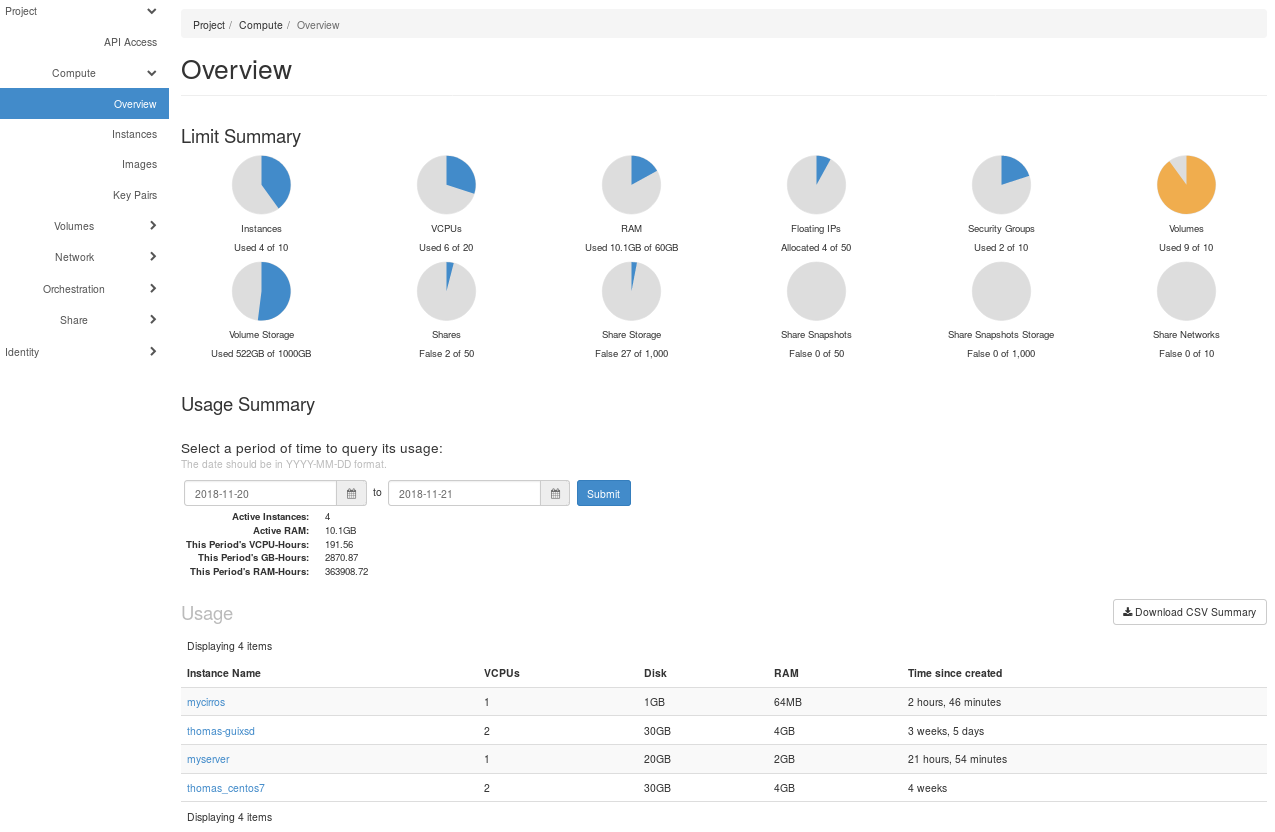
\includegraphics[scale=0.3]{img/tab-compute-overview.png}
\end{center}

\section*{OpenStack dashboard - Project
  tab}\label{openstack-dashboard---project-tab}
Resources (instances, data volumes, networks, \ldots) in OpenStack are
organized into different projects, and every user is a member of one
or more projects.  Every project member has full access to all of the
project's resources.

From the Project tab, you can access the following categories:
\begin{itemize}
\item
  API Access: View API endpoints.
\end{itemize}

\subsection*{\texorpdfstring{Compute
tab}{Compute tab}}\label{compute-tab}

\begin{itemize}
\item
  Overview: View reports for the project.
\item
  Instances: View, launch, create a snapshot from, stop, pause, or
  reboot instances, or connect to them through VNC.
\item
  Images: View images and instance snapshots created by project users,
  plus any images that are publicly available. Create, edit, and delete
  images, and launch instances from images and snapshots.
\item
  Key Pairs: View, create, edit, import, and delete key pairs.
\end{itemize}

\subsection*{\texorpdfstring{Volumes
tab}{Volumes tab}}\label{volumes-tab}

\begin{itemize}
\item
  Volumes: View, create, edit, and delete volumes.
\item
  Backups: View, create, edit, and delete backups.
\item
  Snapshots: View, create, edit, and delete volume snapshots.
\item
  Consistency Groups: View, create, edit, and delete consistency groups.
\item
  Consistency Group Snapshots: View, create, edit, and delete
  consistency group snapshots.
\end{itemize}

\subsection*{\texorpdfstring{Network
tab}{Network tab}}\label{network-tab}

\begin{itemize}
\item
  Network Topology: View the network topology.
\item
  Networks: Create and manage public and private networks.
\item
  Routers: Create and manage routers.
\item
  Security Groups: View, create, edit, and delete security groups and
  security group rules..
\item
  Floating IPs: Allocate an IP address to or release it from a project
\end{itemize}

\subsection*{\texorpdfstring{Orchestration
tab}{Orchestration tab}}\label{orchestration-tab}

\begin{itemize}
\item
  Stacks:
\item
  Resource types:
\item
  Template versions:
\item
  Template generator:
\end{itemize}

\subsection*{\texorpdfstring{Shares
tab}{Shares tab}}\label{shares-tab}

\begin{itemize}
\item
  Shares:
\item
  Share snapshots:
\item
  Share networks:
\item
  Security services:
\item
  Share groups:
\item
  Share group snapshots:
\end{itemize}

\section*{OpenStack dashboard - Identity
tab}\label{openstack-dashboard---identity-tab}

From the Identity tab, you can access the following categories:

\begin{itemize}
\item
  Projects: View, create, assign users to, remove users from, and delete
  projects.
\item
  Users: View, create, enable, disable, and delete users.
\end{itemize}

%%% Local Variables:
%%% mode: latex
%%% TeX-master: "intro-OpenStack"
%%% End:
